\vspace{-0.5em}
\section{Introduction}
Pre-computing views of a database, also known as materialization, is an extensively studied approach to reduce query latency on large data \cite{LarsonY85, gupta1995maintenance, chirkova2011materialized}. 
Materialized Views (MVs) are now supported by all major commercial vendors.
However, as with any pre-computation or caching, the key challenge in using MVs is maintaining their freshness as base data changes.
While there has been substantial work in incremental maintenance of MVs \cite{chirkova2011materialized, DBLP:journals/vldb/KochAKNNLS14}, eager maintenance (i.e., immediately applying updates) is not always feasible.

In real-time analytics applications, such as monitoring or visualization \cite{rainbird, DBLP:journals/cgf/LiuJH13}, analysts may create many MVs by slicing or aggregating over different dimensions.
An eager maintenance strategy would mean that every incoming transaction requires updating all affected MVs, and thus, each additional MV potentially reduces the available transaction throughput.
%Even with recently proposed optimizations such as DBToaster by Koch et al. \cite{DBLP:journals/vldb/KochAKNNLS14}, the cost of simultaneously maintaining multiple MVs can be very significant.
This problem becomes significantly harder when the views are distributed and computational resources are contended by other tasks.
%In fact, many commercial vendors caution against eager maintenance of MVs that join mutliple tables or have selective aggregates \cite{vendors}.
As a result, in production environments, it is common to batch updates together to amortize overheads \cite{chirkova2011materialized}.
Batch sizes are set according to system constraints, and can vary from a few seconds to even nightly.  

While increasing the batching period gives the user more flexibility to schedule around system constraints, a disadvantage is that MVs are stale between maintenance periods.
%As a result, queries using those MVs can return incorrect answers in the interim.
Other than an educated guess based on past data, in general, the user has no way of knowing how incorrect their query results are.
Some types of views and query workloads can be sensitive to even a small number of base data updates, for example, if updates disproportionately affect a subset of frequently queried rows.
Thus, any amount of staleness is potentially dangerous, and this presents us a dichotomy between facing the cost of eager maintenance or coping with consequences of unknown inaccuracy.
In this paper, we explore an intriguing middle ground, namely, for aggregate queries, we can derive a bounded approximation for the correct answer for a fraction of the maintenance cost.
With a small amount of up-to-date data, we can correct for the query result error induces by staleness and improve query result accuracy.


%This observation leads us to the main insight behind our work; namely, that a data cleaning approach can be applied to mitigate the negative impacts of deferred MV maintenance.

\begin{figure}[t] \vspace{-2em}
\centering
 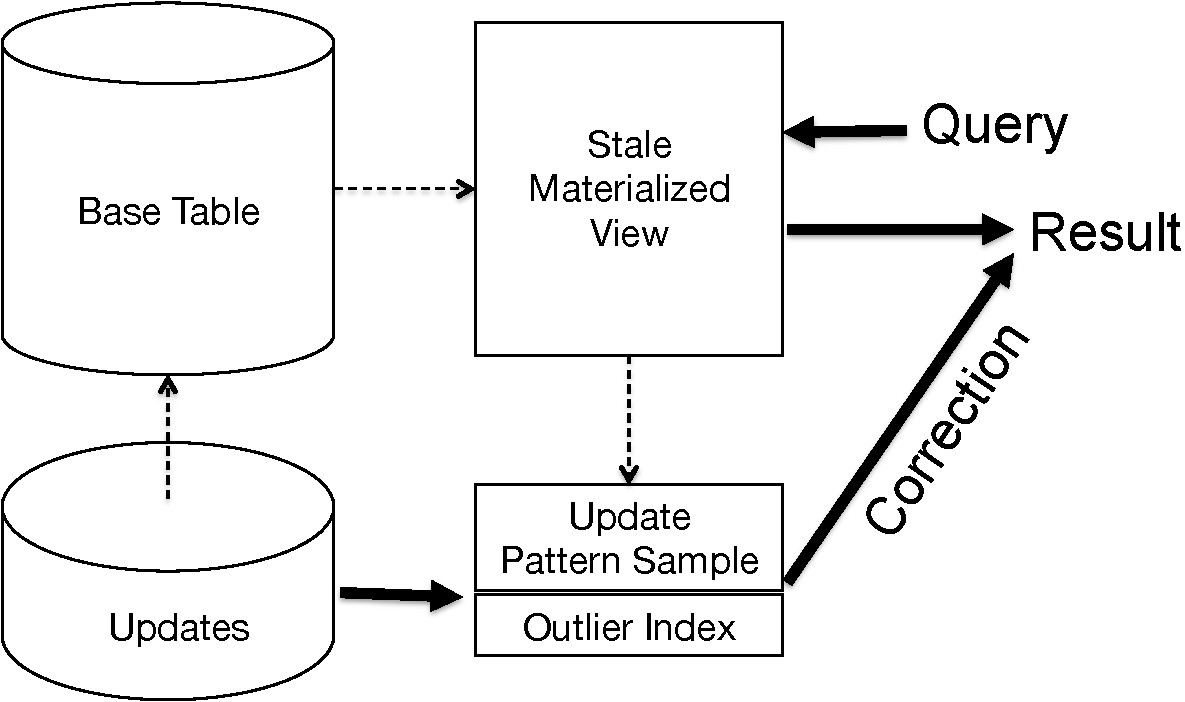
\includegraphics[scale=0.25]{figs/sys-arch.pdf} \vspace{-.25em}
 \caption{Deferred maintenance can lead to stale MVs which have incorrect, missing, and superfluous rows. In \svc, we pose this as a data cleaning problem and show that we can use a sample of clean (up-to-date) rows from an MV to correct inaccurate query results on stale views.\label{sys-arch}}\vspace{-1.75em}
\end{figure}

Our method relies on modeling query answering on stale MVs as a data cleaning problem.
A stale MV has incorrect, missing, or superfluous rows, which are problems that have been studied in the data cleaning literature (e.g., see Rahm and Do for a survey\cite{rahm2000data}).
Increasing data volumes have led to development of new, efficient sampling-based approaches for coping with dirty data.   
In our prior work, we developed the SampleClean framework for scalable aggregate query processing on dirty data \cite{wang1999sample}.
Since data cleaning is often expensive, we proposed cleaning a sample of data and using this sample to improve the results of aggregate queries on the full dataset.
Since stale MVs are dirty data, an approach similar to SampleClean raises a new possibility of using a sample of ``clean'' rows in the MV to return more accurate query results.

\svcfull (\svc illustrated in Figure~\ref{sys-arch}) provides a framework that approximates aggregate queries on a stale MV.
We calculate a relational expression that materializes a uniform sample of up-to-date rows.
This expression can be interpreted as ``cleaning" a stale sample of rows.
We use the clean sample of rows to estimate a result for an aggregate query on the view.
The estimates from this procedure, while approximate, reflect the most recent data. 
Approximation error is more manageable than staleness because: (1) the uniformity of sampling allows us to apply theory from statistics such as the Central Limit Theorem to give tight bounds on approximate results, and (2) the approximate error is parametrized by the sample size which the user can control trading off accuracy for computation.
%\svc is complementary to existing deferred maintenance approaches.
%When the MVs become stale between maintenance batches, we apply \svc for a far smaller cost than having to maintain the entire view but still get approximate, up-to-date answers.

%Both MVs and queries can be complex.
However, the MV setting presents new challenges that we did not consider in prior work.
To summarize our contributions:
\begin{enumerate}[noitemsep]
\item We propose a hashing-based technique that efficiently materializes an up-to-date sample view.
\item We process queries on this view by applying techniques proposed in data cleaning, but significantly extending them to a broader class of queries. Expanding the class of queries results in new challenges in bounding these estimates in confidence intervals. To address this challenge, we also derive a statistical bootstrap estimator to calculate bounds.
\item We apply an outlier indexing technique to reduce sensitivity to skewed datasets. Outlier indexing has not been applied in the MV setting, and we propose an index push-up algorithm that allows us to propagate the outliers to derived relations.
\end{enumerate} 
%\end{itemize}

The paper is organized as follows: 
In Section~\ref{sec-background}, we give the necessary background for our work.
Next, in Section~\ref{sec-arch}, we formalize the problem.
In Sections~\ref{sampling} and~\ref{correction}, we describe the sampling and query processing of our technique.
In Section~\ref{outlier}, we describe the outlier indexing framework.
Then, in Section~\ref{exp}, we evaluate our approach.
Finally, we discuss Related Work in Section~\ref{related}.
In Section~\ref{sec:disc}, we discuss the limitations and future opportunities of our approach, and we present our Conclusions in Section~\ref{conclusion}.
%Full versions of our proofs and experimental details are available in our extended technical report \cite{technicalReport}.
